\chapter{Hintergrund}\label{ch:hintergrund}
%Begriffsklärung, Mathematische Grundlagen und grundlegende Algorithmen
%Wenn Sie mehrere bekannte Verfahren/Algorithmen in ihrer Arbeit verwenden und verketten, sollten sie die Verfahren hier zunächst erklären, so dass der Hauptteil später nicht permanent von Erklärungen einzelner Algorithmen unterbrochen wird. Auch mathematische Grundlagen können hier kurz zusammengefasst werden.
Im Folgenden wird das Konzept des \textit{kontextzentrischen sozialen Netzes} erläutert, das dieser Arbeit zu Grunde liegt. Anschließend werden mengentheoretische und probabilistische Grundlagen und Verfahren sowie Daten- und Indexstrukturen dargestellt, die Eingang in diese Arbeit gefunden haben. Es wird erläutert, inwiefern sie für das soziale Online-Netz AMBIENCE relevant sind oder darin verwendet werden. 
\section{Kontextzentrische soziale Netze}\label{sec:kontext}
Wie eingangs dargestellt lässt sich mit Zunahme der mobilen Endgeräte und dem Erfolgszug des Smartphones eine Tendenz beobachten, die in bestehenden sozialen Online-Netzwerken wenig abgebildet wird: Weg von adressbasiertem Routing und Ende-zu-Ende-Kommunikation hin zu \textit{context-awareness} und \textit{information-centric networking}. 

Der Begriff context-awareness wurde von Schilit et al. 1994 geprägt und bezeichnet die Nutzung von Kontextinformationen als Informationsquelle für Anwendungen und Netzwerke\footnote{Vgl. \cite{Schilit1994}.}. Information-centric networking (ICN) bezeichnet ein neuartiges Konzept für Netzwerke, die nicht auf Ende-zu-Ende- oder Sender/Empfänger-Kommunikation basieren, sondern auf den im Netzwerk vorhandenen Informationen\footnote{Vgl. \cite{Ahlgren2012} für eine ausführliche Darstellung.}. 
Der Begriff \textit{Kontext} im Zusammenhang mit interaktiven Anwendungen wurde bereits in den 90er Jahren geprägt. In der klassischen Definition von Dey und Abowd bedeutet Kontext 
\begin{quote}
[...] any information that can be used to characterize the situation of an entity. An entity is a person, place, or object that is considered relevant to the interaction between a user and an application including the user and application themselves\footnote{\cite{Dey1999}: 306f..}. 
\end{quote}
Diese Definition wird für soziale Online-Netze eingegrenzt: 
\begin{quote}
Context is any information that can be used to infer aspects of the surroundings of an entity in a way, in which some applications may have interest. Surroundings include all information that could possibly impact the behaviour of the entity\footnote{\cite{Werner2015}: 2.}.
\end{quote}
Ein kontextzentrisches soziales Netz ist also ein soziales Online-Netz, das auf Kontext-Variablen wie Ort und Zeit als Informationsquellen basiert und in der Regel dezentral organisiert ist (z.B. mit einer Peer-to-Peer- statt einer Client/Server-Architektur). Kommunikation beruht darin allein auf Kontext-Ähnlichkeit, nicht auf Online-Freundschaft: 
\begin{quote}
A context-centric online social network is an online social network in which the edges of the social graph are defined from context information and context matching algorithms. An edge between two profiles exists for a fixed information object if and only if the two profiles share the relevant context as defined by the publisher\footnote{\cite{Werner2015}: 4.}.
\end{quote}
\subsection{AMBIENCE}\label{sec:ambience}
AMBIENCE ist ein soziales Online-Netzwerk, das 2015 als Prototyp implementiert wurde und sich an diesem neuen Paradigma orientiert. Die vorliegende Arbeit hat das Ziel, einen spezifischen Aspekt des Netzwerks zu optimieren, nämlich die Organisation der Nachrichten an einem Host für \textit{k}-nächste-Nachbarn-Anfragen. Nachrichten und Anfragen werden in AMBIENCE als Bloom-Filter kodiert. Bei einer Anfrage wird also ein Anfrage-Filter mit einer Menge von Bloom-Filtern verglichen, die an einem Host gespeichert sind. Aktuell werden die Filter dort einfach als unsortierte Liste gespeichert. Die Laufzeit für \textit{k}-nächste-Nachbarn-Anfragen an einen Host mit \textit{n} Filtern liegt damit in $O(n^2)$. Dieses Laufzeitverhalten gilt es zu optimieren, wenn das Netzwerk wachsen und über den Status eines Prototypen hinaus erfolgreich sein soll. 
\section{Bloom-Filter}\label{sec:bloom}
Ein Bloom-Filter ist eine probabilistische Datenstruktur zur Beschreibung von Mengen, die in der ursprünglichen From 1970 von Burton H. Bloom eingeführt wurde\footnote{Vgl. \cite{Bloom1970}.}. Er besteht aus einem Bit-Array der festen Länge \textit{m}, dessen Elemente zunächst alle auf 0 gesetzt sind. Das Einfügen von Informationsobjekten basiert auf der Berechnung einer festen Anzahl \textit{k} unabhängiger Hashfunktionen, die positive Werte kleiner als \textit{m} annehmen. Soll ein Objekt in den Filter eingefügt werden, werden seine Hashwerte berechnet und die die entsprechenden Bits im Filter gesetzt\footnote{Vgl. \cite{Broder2004}: 487.}. 

Die Hashwerte werden verwendet, um Anfragen auf dem Filter auszuführen. Ist ein Objekt im Filter enthalten, sind seine Bits gesetzt worden, d.h. man kann eine Anfrage nach seinen Hashwerten durchführen und so mit großer Wahrscheinlichkeit ermitteln, ob es in den Filter eingefügt wurde: Sind ein oder mehrere Bits des Anfrageobjekts nicht gesetzt, so ist das Element mit Sicherheit nicht vorhanden. Es gibt also keine falsch negativen Antworten. Allerdings kann es sein, dass ein Element nicht in den Filter eingefügt wurde, obwohl alle seine Bits gesetzt sind (falsch positive Antworten). Grund dafür ist die Kollisionseigenschaft von Hashfunktionen, die ein großes Universum von Elementen auf einen sehr viel kleineren Wertebereich, hier die Länge des Bloom-Filters, abbilden. Es kann somit zu Kollisionen zwischen unterschiedlichen Informationsobjekten bzw. ihren charakteristischen Hashwerten kommen. Die Falsch-Positiv-Rate eines Bloom-Filters ist abhängig von \textit{m}, \textit{k} und der Anzahl der eingefügten Elemente \textit{n} und lässt sich berechnen als\footnote{Vgl. ebd. für eine umfassende Darstellung.}
\[f = \left(1 - \left(1-\frac{1}{m}\right)^{kn}\right)^k.\]
% \newpage
% \noindent
% \enlargethispage{\baselineskip}
Aus der Kollisionseigenschaft folgt auch, dass ein einmal eingefügtes Objekt nicht mehr aus einem Bloom-Filter gelöscht werden kann, weil das offensichtlich zu falsch negativen Ergebnissen für andere Objekte führen könnte. 
\begin{figure}[hpbt]
  \centering
  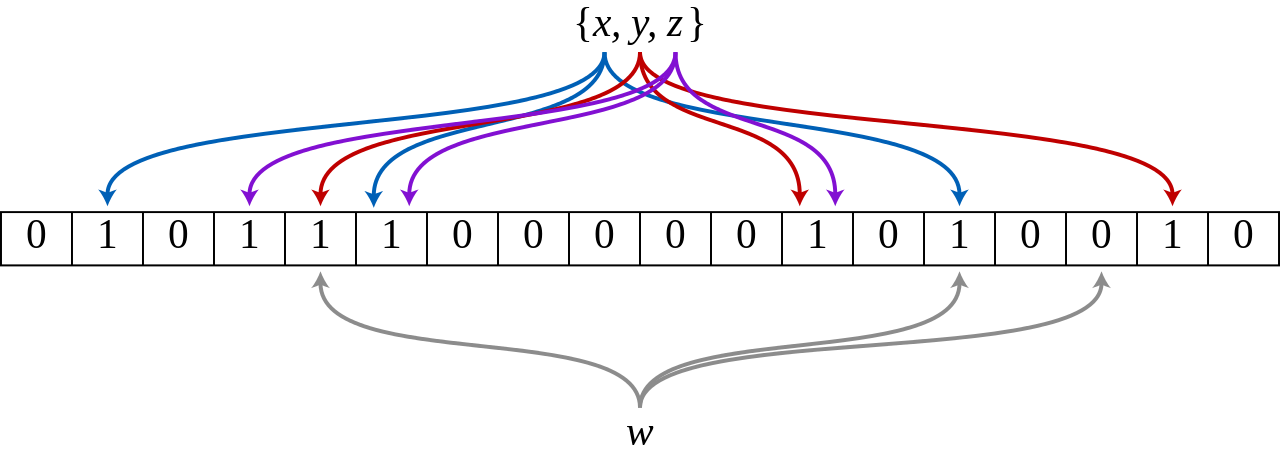
\includegraphics[width=0.8\textwidth]{pictures/1280px-Bloom_filter.png}\\
  \caption[Bloomfilter-Beispiel, Bildnachweis: \url{https://commons.wikimedia.org/wiki/File:Bloom_filter.svg}.]{Beispiel für einen Bloomfilter, in den die Objekte \textit{x}, \textit{y} und \textit{z} eingefügt wurden. Das Objekt \textit{w} ist nicht im Filter vorhanden.}\label{fig:pic0}
\end{figure}
\subsection{Distanzmaße}\label{sec:distanzmasse}
Um die Ähnlichkeit zweier Mengen zu ermitteln, werden verschiedene Distanzmetriken oder Ähnlichkeitsmaße eingesetzt. Um Bloom-Filter miteinander zu vergleichen und insbesondere für die \textit{k}-nächste-Nachbarn-Suche muss ein geeignetes Ähnlichkeitsmaß zur Anwendung kommen. Bayardo et al. verwenden dazu die \textit{Kosinus-Ähnlichkeit}\footnote{Vgl. \cite{Bayardo2007}.}. Sakuma und Sato definieren die Ähnlichkeit von Bloom-Filtern über die Anzahl gleicher 1-Bits\footnote{Vgl. \cite{Sakuma2011}: 321.}. Ist diese für zwei Anfragefilter identisch, werden die Bit-Arrays negiert und die Anzahl gleicher 0-Bits verglichen. 

AMBIENCE verwendet eine Abschätzung der \textit{Jaccard-Distanz} zur Ermittlung der Ähnlichkeit von Bloom-Filtern. Die Jaccard-Distanz zwischen zwei Mengen \textit{A} und \textit{B} ist definiert als 
\[J_{\delta}(A,B) = 1 - J(A,B) = \frac{|A\cap B| - |A\cup B|}{|A\cup B|}, \]
wobei 
\[J(A,B) = \frac{|A\cap B|}{|A\cup B|}\] den \textit{Jaccard-Koeffizienten} bezeichnet. Die Jaccard-Distanz nimmt Werte im Bereich $\left[0,1\right]$ an. Identische Mengen haben eine Jaccard-Distanz von 0, Mengen ohne gemeinsame Elemente haben eine Jaccard-Distanz von 1. 
Für Bloom-Filter lässt sich die Jaccard-Distanz analog berechnen. Die Vereinigungsmenge zweier Bloom-Filter \textit{F} und \textit{G} lässt sich als bitweises logisches Oder, die Schnittmenge als bitweises logisches Und repräsentieren. Auch hier nimmt die Jaccard-Distanz offensichtlich Werte zwischen 0 und 1 an. Je ähnlicher die Filter sind, desto kleiner ist ihre Jaccard-Distanz. 
Die Jaccard-Distanz zwischen Bloom-Filtern ist, anders als die von Sakuma und Sato verwendete Distanz-Metrik, nicht transitiv in dem Sinne, dass zwei Filter, die beide eine geringe Jaccard-Distanz zu einem dritten Filter aufweisen, untereinander nicht ähnlich sein müssen. Man betrachte z.B. die Filter \textit{F1}, \textit{F2} und \textit{F3} mit folgenden Werten: 
\begin{figure}
  \centering
  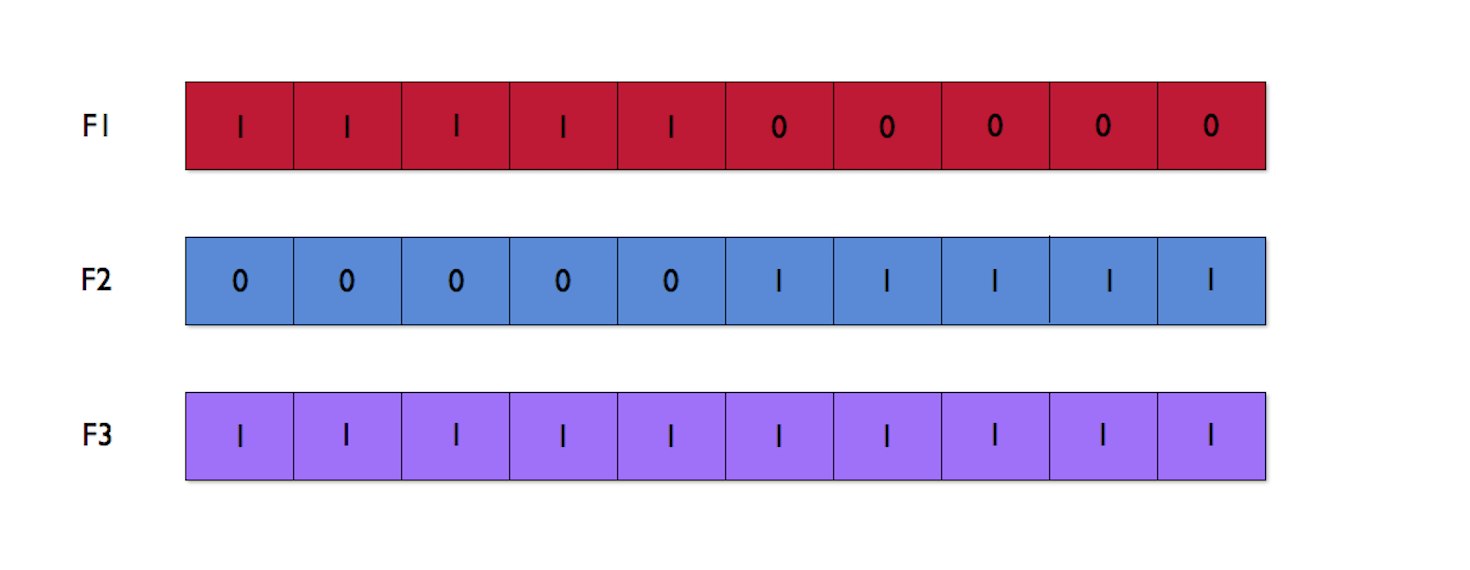
\includegraphics[width=1.0\textwidth]{pictures/filters.png}\\
  \caption[Jaccard-Distanzen zwischen Bloom-Filtern]{Jaccard-Distanzen zwischen Bloom-Filtern.}\label{fig:pic1}
\end{figure}
\noindent
Die Jaccard-Distanzen zwischen \textit{F1}, \textit{F2} und \textit{F3} betragen somit: 
\[J_{\delta}(F1,F3) = 1 - J(F1,F3) = 1 - \frac{|F1\cap F3|}{|F1\cup F3|} = 1 - \frac{5}{10} = 0.5\]
\[J_{\delta}(F2,F3) = 1 - J(F2,F3) = 1 - \frac{|F2\cap F3|}{|F2\cup F3|} = 1 - \frac{5}{10} = 0.5\]
\[J_{\delta}(F1,F2) = 1 - J(F1,F2) = 1 - \frac{|F1\cap F2|}{|F1\cup F2|} = 1 - 0 = 1\]
Daran wird deutlich: Obwohl \textit{F1} und \textit{F2} jeweils die Hälfte der Elemente mit \textit{F3} gemeinsam haben, lässt sich daraus kein Wert für die Ähnlichkeit zwischen \textit{F1} und \textit{F2} ableiten. Sie sind sich im Gegenteil maximal unähnlich. 
\subsection{Teil- und Obermengenbeziehung}\label{sec:mengenbeziehungen}
Will man Bloom-Filter z.B. nach Ähnlichkeit gruppieren, kann man stattdessen Teil- und Obermengenbeziehungen zwischen ihnen betrachten. Die Teilmengenbeziehung zwischen zwei Bloom-Filtern sei hier wie folgt definiert: 
\begin{quote}
Ein Bloom-Filter \textit{F} ist \textbf{\textit{Teilmenge}} eines Bloom-Filters \textit{G}, wenn darin mindestens die gleichen 0-Bits gesetzt sind wie in \textit{G} (und möglicherweise weitere, zusätzliche 0-Bits).
\end{quote}
Die Obermengenbeziehung zwischen zwei Bloom-Filtern sei hier wie folgt definiert: 
\begin{quote}
Ein Bloom-Filter \textit{F} ist \textbf{\textit{Obermenge}} eines Bloom-Filters \textit{G}, wenn darin mindestens die gleichen 1-Bits gesetzt sind wie in \textit{G} (und möglicherweise weitere, zusätzliche 1-Bits).
\end{quote}
Der maximal gefüllte Filter, in dem alle Bits gesetzt sind, ist damit Obermenge aller Filter derselben Länge (auch von sich selbst). Der leere Filter ist die (triviale) Teilmenge aller Filter derselben Länge (auch von sich selbst). Teil- und Obermengen sind Umkehrungen voneinander, d.h. wenn \textit{F} Teilmenge von \textit{G} ist, folgt daraus, dass \textit{G} Obermenge von \textit{F} ist, und umgekehrt.  

Zwischen den Bloom-Filtern in Abb. \ref{fig:pic1} bestehen folgende Teil- und Obermengenbeziehungen: \textit{F1} und \textit{F2} sind Teilmengen von \textit{F3}. \textit{F3} ist Obermenge von \textit{F1} und \textit{F2}. Zwischen den maximal unähnlichen Filtern \textit{F1} und \textit{F2} bestehen keine Teil- und Obermengenbeziehungen. 
\begin{figure}[hpbt]
  \centering
  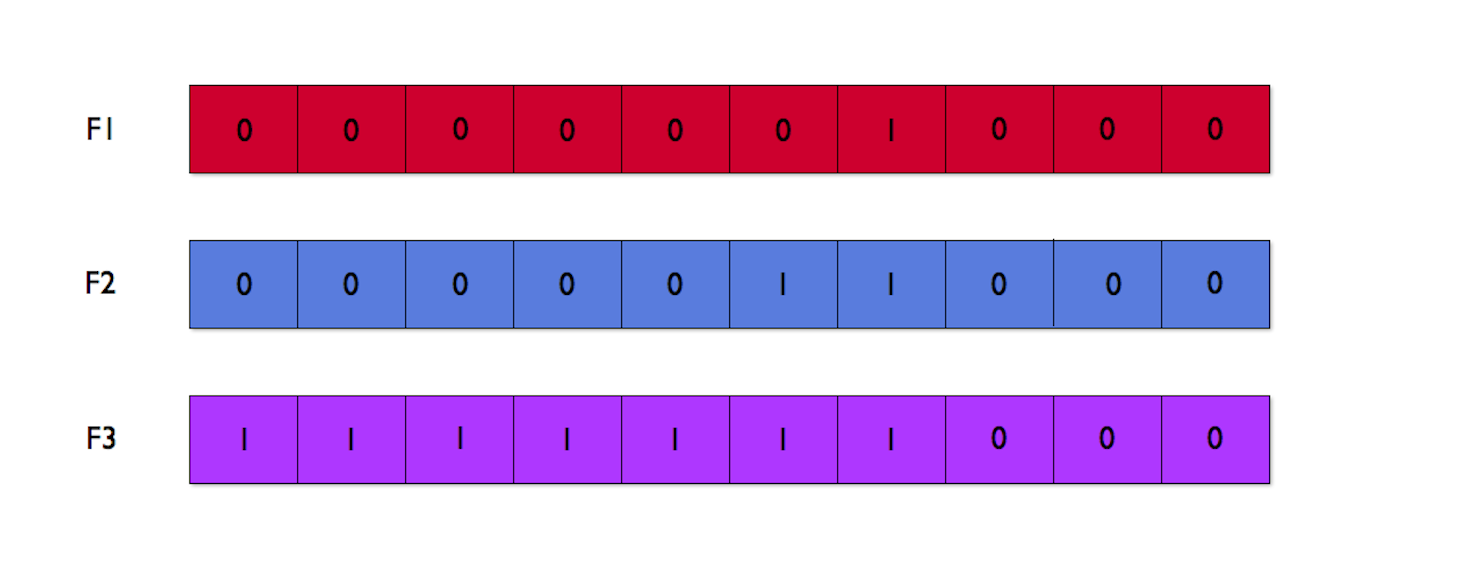
\includegraphics[width=1.0\textwidth]{pictures/distances.png}\\
  \caption[Teil- und Obermengenbeziehungen zwischen Bloom-Filtern]{Teil- und Obermengenbeziehungen zwischen Bloom-Filtern.}\label{fig:pic2}
\end{figure}

\noindent
Teil- und Obermengenbeziehung sind außerdem transitiv, was an Abb. \ref{fig:pic2} deutlich wird: \textit{F1} ist Teilmenge von \textit{F2}, damit auch Teilmenge von \textit{F3}. \textit{F3} ist Obermenge von \textit{F2}, damit auch Obermenge von \textit{F1}. 

Teil- und Obermengenbeziehungen sind also im Gegensatz zur Jaccard-Distanz dazu geeignet, transitive Ähnlichkeitsbeziehungen zwischen Bloom-Filtern abzubilden. Diese Eigenschaft spielt eine zentrale Rolle im hier entwickelten Verfahren, das in Kap. \ref{ch:implementierung} ausführlich dargestellt wird. 
\subsection{Hashfunktionen}\label{sec:hashfunktionen}
Die Frage nach den idealen Hashfunktionen für einen Bloom-Filter ist nicht eindeutig zu beantworten\footnote{Vgl. \cite{Broder2004}: 487.}. Grundsätzlich muss zwischen kryptografischen Hashfunktionen wie MD5 und SHA und gewöhnlichen Hashfunktionen wie Murmur- oder Jenkins-Hashfunktionen unterschieden werden. Die Berechnung von kryptografischen Hashfunktionen dauert in der Regel länger, dafür haben sie bestimmte Eigenschaften wie eine hohe Kollisionsresistenz und Gleichverteilung der Ergebniswerte. 

Werden Bloom-Filter z.B. zum schnellen Nachschlagen in großen, verteilten Datenbanken eingesetzt, wird auf die kryptografischen Eigenschaften zu Gunsten des verminderten Rechenaufwandes verzichtet. Das NoSQL-Datenbanksystem Cassandra und das Hadoop-Framework für skalierte, verteilt arbeitende Software verwenden beispielsweise Bloom-Filter in Kombination mit Murmur- und Jenkins-Hashfunktionen. Darüber hinaus ist MD5 für Bloom-Filter weit verbreitet. Die Murmur-Hashfunktionen weisen gleichzeitig gute Verteilungseigenschaften auf und lassen sich vergleichsweise schnell berechnen, weswegen sie generell für den Einsatz in Bloom-Filtern empfohlen werden\footnote{Vgl. \url{http://spyced.blogspot.de/2009/01/all-you-ever-wanted-to-know-about.html}.}. AMBIENCE verwendet Murmur-Hashfunktionen zur Generierung der Bloom-Filter. Für die eigene Implementierung wurde der Murmur2-Hash verwendet\footnote{Vgl. \url{https://sites.google.com/site/murmurhash/MurmurHash2.cpp} für den Quellcode.}.  
\subsection{Bloom-Filter-Varianten und Anwendungen}\label{sec:bloom-anwendungen}
Wegen ihres geringen Speicherbedarfs und einfachen Implementierung erfreuen sich Bloom-Filter in unterschiedlichsten Versionen großer Beliebtheit. Wichtige Varianten sind z.B. \textit{Attenuated Bloom Filter}, \textit{Counting Bloom-Filter} und \textit{Compressed Bloom Filter}. Ein Counting Bloom-Filter benötigt mehr Speicherplatz als ein klassischer Bloom-Filter, dafür können Objekte wieder daraus entfernt werden\footnote{Vgl. \cite{Fan2000}.}. Komprimierte Bloom-Filter werden eingesetzt, wenn Bloom-Filter als Nachrichten mit begrenzter Länge versendet werden oder die übertragene Datenmenge minimiert werden soll\footnote{Vgl. \cite{Mitzenmacher2002}.}. Attenuated Bloom-Filter\footnote{Vgl. \cite{Sakuma2011}: 316 und 318.} können als Array von Bloom-Filtern betrachtet werden und können z.B. in einem Netzwerk Informationen darüber enthalten, welche Dienste an einem anderen Knotenverfügbar sind. Besonders häufig kommen Bloom-Filter in verteilten Anwendungen und Netzwerkdiensten zum Einsatz\footnote{Vgl. \cite{Broder2004} für eine ausführliche Darstellung.}. 

Neben Hadoop und Cassandra werden Bloom-Filter in unzähligen, zum Teil hoch skalierenden Anwendungen eingesetzt. Weitere Beispiele sind der quelloffene Webproxy Squid und der Chrome-Browser, wo Bloom-Filter zum schnellen Nachschlagen als bösartig eingestufter Webseiten verwendet werden. Broder und Mitzenmacher formulieren das Bloom-Filter-Prinzip wie folgt: 
\begin{quote}
Wherever a list or set is used, and space is at a premium, consider using a Bloom filter if the effect of false positives can be mitigated\footnote{\cite{Broder2004}: 486.}.
\end{quote}
\section{Indexstrukturen}\label{sec:indexstrukturen}
Zur effizienten Bearbeitung von Anfragen und Operationen kommen in der internen Schicht von Datenbanksystemen spezielle Datenstrukturen und Speicherverfahren zum Einsatz. Sie werden \textit{Indexstrukturen} genannt und organisieren die Daten an Hand von Indizes, um die gewünschten Operationen zu unterstützen\footnote{Trotz der großen Verbreitung von Indexstrukturen in Datenbanksystemen scheinen in der Literatur keine überblicksartigen Darstellungen zu existieren. Der aktuelle Abschnitt stützt sich daher im Wesentlichen auf das Skript zur Vorlesung \textit{Anfragebearbeitung und Indexstrukturen in Datenbanksystemen} im Wintersemester 2013/2014 an der Ludwig-Maximilians-Universität München (vgl. \cite{Kriegel1994--2013}).}.

Ein \textit{Index} oder \textit{Verzeichnis} einer Datei enthält Informationen über ihre Struktur, wobei mit "`Datei"' in diesem Zusammenhang eine komplette Datenstruktur gemeint ist, also z.B. ein Suchbaum oder ein Array. Indexstrukturen lassen sich danach klassifizieren, wie sie die Daten organisieren: 
\begin{enumerate}
	\item \textit{Daten-organisierende Indexstrukturen} werden zur Organisation der tatsächlich anfallenden Daten eingesetzt -- meist in Form von \textit{Suchbäumen}. 
	\item \textit{Raum-organisierende Indexstrukturen} werden zur Organisation des Speichers eingesetzt, in dem die Daten gehalten werden. Sie verwenden vor allem \textit{dynamische Hashverfahren}. 
	\item \textit{Hybride Indexstrukturen} sind eine Kombination der vorgenannten Klassen und basieren auf \textit{Hashbäumen}.   
\end{enumerate}
Anforderungen an eine gute oder effektive Indexstruktur können sein: 
\begin{itemize}
	\item \textit{Effiziente Suche:} Eine Suchanfrage auf der Indexstruktur soll in optimaler Zeit ein Ergebnis liefern. D.h. die Anfrage soll in möglichst wenig Schritten an die Seite oder Seiten weiter geleitet werden, die die angefragten Daten enthält oder enthalten.
	\item \textit{Dynamisches Einfügen, Modifizieren und Löschen von Datensätzen:} Die zu organisierende Datenmenge verändert sich möglicherweise über die Zeit, was durch die Indexstruktur widergespiegelt und unterstützt werden muss.  
	\item \textit{Erhalt der lokalen Ordnung:} Falls es Datensätze gibt, deren Schlüssel in der angewandten Ordnungsrelation (z.B. die Kleiner-Gleich-Ordnung) aufeinander folgen, sollte die Indexstruktur das widerspiegeln. Diese Eigenschaft wird von Suchbäumen erfüllt, nicht aber von linearen Hashverfahren. Die Wahl bzw. Implementierung der Indexstruktur muss also nach dem jeweiligen Anwendungsfall erfolgen. 
	\item \textit{Speichereffizienz:} Effiziente Speichernutzung ist vor allem in der realen Welt und in hoch skalierenden Anwendungen von zentraler Bedeutung. 
\end{itemize}
Weitere Anforderungen beinhalten \textit{Machbarkeit} und \textit{Implementierungskosten}. Für die hier vorgestellte Implementierung wird darauf nicht näher eingegangen.  
\cite{Ottmann2012}
\subsection{B+-Bäume}\label{sec:b+bäume}
\cite{Knuth1998}	
\subsection{Doppelt verkettete Listen}\label{sec:listen}	


%\subsection{Tabellen}
%Es gibt schöne Möglichkeiten Tabellen einzubinden wie z.B. Tabelle \ref{tab:CommonParameterSettings}.
%\begin{center}
%\begin{table}[htbp]
%{\small
%\begin{center}
%\begin{tabular}[center]{lrlc}
%\toprule
%Parameter & Value & (Unit) & Available for Chord \\
%\midrule
%Query timeout & 10 & seconds & $\surd$ \\
%Republish timeout & 300 & seconds & $\surd$ \\ % explain this value...
%Stabilize timeout & 5 & seconds & $\surd$ \\
%Fix fingers timeout & 30 & seconds & $\surd$ \\
%Message timeout & 1 & second & $\surd$ \\
%Connect timeout & 10 & seconds & $\surd$ \\
%Ping superpeer timeout & 5 & seconds & $\times$ \\
%Cost-Optimality estimation timeout & 20 & seconds & $\times$ \\
%Significance for change in number of superpeers & 10 & percent & $\times$ \\
%Significance for change in estimations  & 10 & percent & $\times$ \\
%Number of permanent superpeers & 32 & nodes & $\times$ \\
%Mean number of peers & 1000 & nodes & $\surd$ \\
%Mean number of lookups per hour & 60 & queries & $\surd$ \\
%Mean number of shared InfoProfiles per node & 20 & & $\surd$ \\
%Identifier space & 16 & bits & $\surd$ \\
%Direct insertion acknowledgment & true & bool & $\times$ \\
%Direct query responses & true & bool & $\times$ \\
%Force query resolution & true & bool & $\surd$  \\
%\bottomrule
%\end{tabular}
%\end{center}
%} % end of tiny
%\caption[Simulation parameter settings]{Common simulation parameter settings.\label{tab:CommonParameterSettings}}
%\end{table}
%\end{center}
%
%\subsection{Bilder}
%Man kann sehr einfach Bilder einbinden so wie z.B. in Abbildung \ref{fig:pic0}.
%\begin{figure}[hpbt]
%  \centering
%  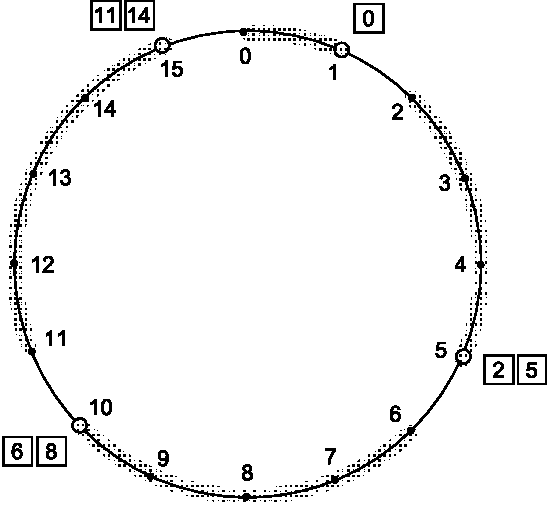
\includegraphics[width=0.4\textwidth]{pictures/pic0}\\
%  \caption[Example of a $4$-bit Chord identifier circle]{Example of a $4$-bit Chord identifier circle.
%  The responsibility ranges for each peer are accentuated in light gray}\label{fig:pic0}
%\end{figure}
%Es lassen sich auch mehrere Bilder nebeneinander platzieren wie z.B. in Abbildung
%\ref{fig:multipic} zu sehen ist.
%\begin{figure}[hpbt]
% \centering
%  %%----start of first subfigure----
%  \subfloat[FIFO size limited to 20 entries]{
%   \label{fig:multipic:a} %% label for first subfigure
%   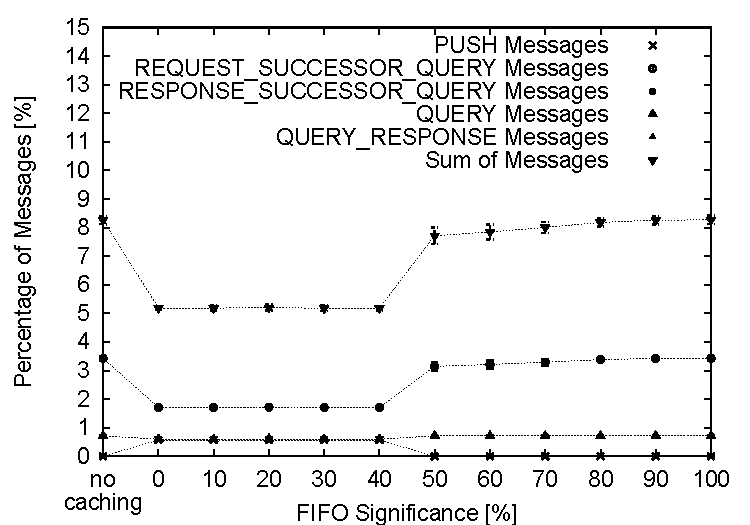
\includegraphics[width=0.48\linewidth]{pic1}}
%  \hspace{0.01\textwidth}
%  %%----start of second subfigure----
%  \subfloat[FIFO size limited to 30 entries]{
%   \label{fig:multipic:b} %% label for second subfigure
%   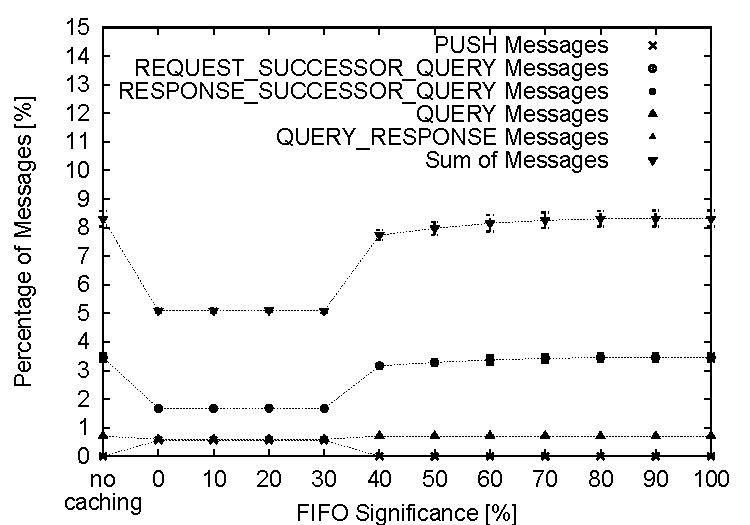
\includegraphics[width=0.48\linewidth]{pic2}}\\[0pt] % horizontal break
%  %%----start of third subfigure----
%  \subfloat[FIFO size limited to 40 entries]{
%   \label{fig:multipic:c} %% label for third subfigure
%   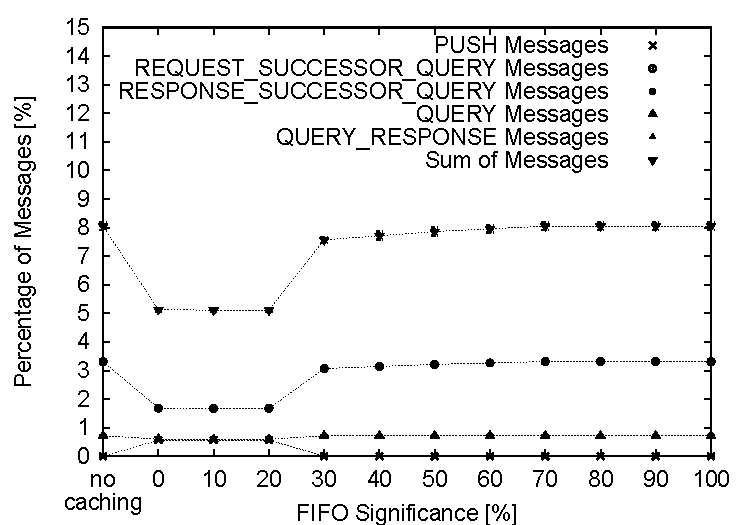
\includegraphics[width=0.48\linewidth]{pic3}}
%  \hspace{0.01\textwidth}
%  %%----start of fourth subfigure----
%  \subfloat[FIFO size limited to 50 entries]{
%   \label{fig:multipic:d} %% label for fourth subfigure
%   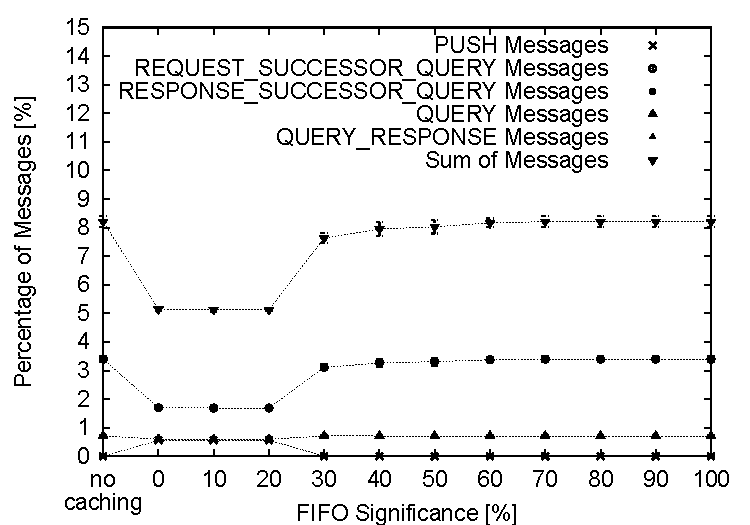
\includegraphics[width=0.48\linewidth]{pic4}}
% \caption[Observed message fractions and 95\% confidence intervals for Chord]{Observed message fractions and 95\% confidence intervals for Chord without the influence of churn. The FIFO capacity varies from 20 (\ref{fig:multipic:a}) -- 50 (\ref{fig:multipic:d}) entries (decadic steps).}
% \label{fig:multipic} %% label for entire figure
%\end{figure}
%
%\subsection{Programm Code}
%Eine elegante Möglichkeit, Programmtext einzubinden, lässt sich mit dem listings-Paket erreichen.
%Das \verb|HelloWorld| Programm aus Listing \ref{lst:hw} hat in Zeile \ref{line:hw3} übrigens einen Programmierfehler.
%\begin{lstlisting}[float=htp,caption=Hello World,label=lst:hw,language=Java, numbers=left, numberstyle=\tiny, stepnumber=2, numbersep=8pt, escapeinside={//@}{@//},backgroundcolor=\color{yellow},xleftmargin=3ex,xrightmargin=1ex]
%public class HelloWorld {
%    public static void main(String[] args) {
%        Syste.out.println("Hello, World"); //@\label{line:hw3}@//
%    }
%}
%\end{lstlisting}